\chapter{Summarising the Posterior Distribution}
The posterior distribution is the full answer to any Bayesian problem. It gives
a complete description of our state of uncertainty about the value(s) of unknown
parameters. From the posterior distribution, we can calculate any probability
we want. For example, if we had a posterior distribution $p(\theta|x)$ and we
wanted to know the probability that $\theta$ is greater than 100, we could do:
\begin{eqnarray}
P(\theta > 100 | x) &=& \int_{100}^\infty p(\theta | x) \, dx.
\end{eqnarray}
We could also do a lot of other things.
However, the posterior distribution is sometimes too much
information for us to think about easily. We need to summarise it to help
communicating our results with others. A giant Bayes' Box, or a million MCMC
samples of the parameter, might technically
contain everything we want, but it's not easy to talk about.

For example, say you were trying to estimate
a parameter, and a colleague asked you to state your uncertainty about the
parameter. Well, your posterior distribution might be complicated, it might
have bumps and wiggles in it, or some other kind of structure.
Figure~\ref{fig:complicated_posterior} shows an example of what a complicated
posterior distribution might look like. If this was your result, your colleague
might not care about all the little wiggles in this plot. They just want to know
the ``big picture'' of your results.
\begin{figure}[h!]
\begin{center}
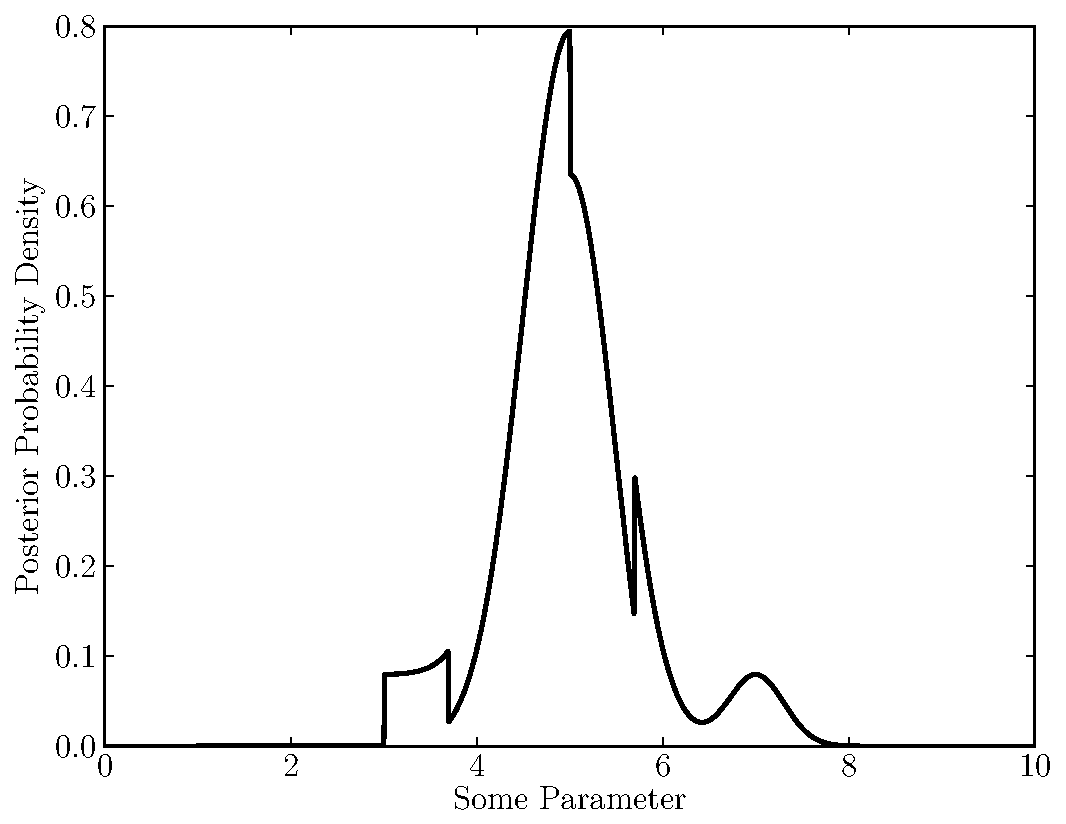
\includegraphics[scale=0.6]{Figures/complicated_posterior.pdf}
\caption{A complicated posterior distribution.\label{fig:complicated_posterior}}
\end{center}
\end{figure}

\begin{framed}
{\bf In descriptive statistics, you often make summaries of a complex data set
(e.g. the mean and the standard deviation) so that you can communicate about
the data set in a concise way. In Bayesian statistics, you often do a similar
thing, but instead of giving a concise description of the data, you give a
concise description of the posterior distribution.}
\end{framed}

\section{Point Estimates}
A ``point estimate'' refers to a single number guess for the value of the parameter.
If you have several parameters, a point estimate would be a single guess for the
value of each parameter (like a single point in a multidimensional space).
If you look at the
posterior distribution plotted in Figure~\ref{fig:complicated_posterior}, you
can see that the true value of the parameter is probably somewhere around 5,
but with some uncertainty. If you were to provide a single number as a guess of
the parameter, you would probably say something close to 5. In statistics, a
single number guess is called an ``estimate'', and is written by putting a
little hat over the name of the parameter. So, by looking at the plot of the
posterior, you could give an estimate like this:
\begin{eqnarray}
\hat{\theta} = 5.
\end{eqnarray}
But there are better things you could do, and I'd bet you know some of them
from previous statistics courses. Here are three methods you could use to
choose a point estimate using the posterior distribution: the posterior mean
(expectation value), the posterior median (the value that divides the probability
in half), and the posterior mode (the value where the posterior PDF has its
peak). This gives the following three possible estimates:
\begin{eqnarray}
\hat{\theta} &=& 4.988 \textnormal{ (the posterior mean)}\\
\hat{\theta} &=& 4.924 \textnormal{ (the posterior median)}\\
\hat{\theta} &=& 4.996 \textnormal{ (the posterior mode)}
\end{eqnarray}
In this example, there's not much of a difference between these three methods.
But in other situations, they can be quite different (this usually happens if
the posterior distribution is skewed, or has multiple modes: you may notice a
strong analogy between this topic and descriptive statistics). Is there a way
to say which one is the {\it best}? It turns out that there is, but that
depends on what you mean by ``best''.

\subsection{A Very Brief Introduction to Decision Theory}
Decision theory is a very important topic. In this course we will use a
{\it tiny} amount of it. Just enough to solve the problem of ``which point
estimate is best?''. If you think about it, this is a bit of a weird question.
{\it The best point estimate is the true value}. Of course it is, how could it
be otherwise? Our problem is that we can't actually implement this suggestion.
We don't know the true value, we only have the posterior distribution
(which is based on all the evidence we have), so we have to do 
the best we can with that.

To think about which decision is the best, the first thing we should do is think
about what decisions are {\it possible}. For estimating a single parameter, any
real number is a possible guess.






\subsection{Computing Point Estimates from a Bayes' Box}
The posterior mean is straightforward. It's the expectation value of the parameter
using the posterior distribution. In R, the code is:
\begin{framed}
\begin{verbatim}
post_mean = sum(theta*post)
\end{verbatim}
\end{framed}
You should also know how to compute this manually from a Bayes' Box, using a
calculator.

The posterior mode is also fairly straightforward. First, we can find the
highest probability in the Bayes' Box. Then we find the values of the parameter
that correspond to this probability.
\begin{framed}
\begin{verbatim}
max_post = max(post)
post_mode = theta[post == max_post]
\end{verbatim}
\end{framed}
Note that, in the case of a tie, {\tt post\_mode} might be a vector, indicating
that there isn't a single mode.



\subsection{Computing Point Estimates from Samples}





\section{Credible Intervals}

\subsection{Computing Credible Intervals from a Bayes' Box}


\subsection{Computing Credible Intervals from Samples}


\section{Confidence Intervals}
In previous stats courses you have probably come across the concept of a
{\it confidence interval}. A confidence interval is a concept in classical
statistics that is somewhat similar to a credible interval in Bayesian statistics.
When people calculate confidence intervals, they usually want to be
able to say that they are 95\% sure that the parameter is in that interval,
given the data. This is what Bayesian credible intervals do, but {\it it is not
what classical confidence intervals do}!

Luckily, a lot of the time, the classical and the Bayesian methods for making
intervals will actually give the same interval. But this isn't always the case!
In lectures we will study an example where the Bayesian credible interval and
the classical confidence interval give completely different results. I wonder
which one will be more sensible?
